\section{Intro}
\scriptsize{Form and meaning pairs} \\
%{\tiny How does the mapping between form and meaning work? Does it work at all?}\\
\scriptsize{Syntax} {\tiny morphosyntactic and POS level}\\
\scriptsize{Semantics} {\tiny mapping of utterances to the “real world”, translation into another language, translation into a universally valid logical form}\\
\scriptsize{Combinatorial structure} {\tiny a small number of meaningless building blocks (phonemes, parts of syllables) combined into an unlimited set of utterances (words and morphemes)}\\
\scriptsize{Compositionality} {\tiny hallmark of human language syntax and semantics, as it enables the infinite use of finite means}\\
\scriptsize{Non-Adjacency} {\tiny non-linearity of syntax, or long-distance dependency, elements of a sentence which depend on each other, do not necessarily
occur next to each other in linear order}
\subsection*{Constituency}
{\tiny basic elements/units (orthographic words) and combinations (phrases)}\\
\scriptsize{Wordhood criterion} {\tiny free occurrence, external mobility and internal fixedness, uninterruptibility, non-selectivity, non-coordinatability, anaphoric islandhood, nonextractability, morphophonological idiosyncrasies, derivations from biuniqueness}\\
\scriptsize{Constituency tests:}\\
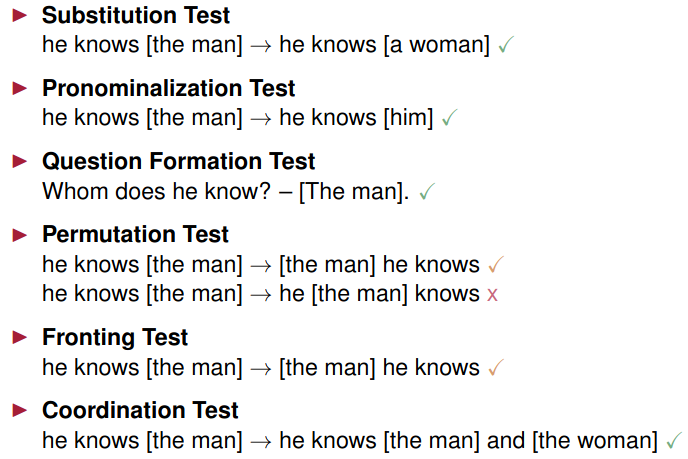
\includegraphics[scale=0.2]{constituency-test.png}\\
\subsection*{POS}
{\tiny classes of words that each lexical item is assigned to according to its morphosyntactic properties. According to Müller (2019: 18) the basic POS are Verb, Noun, Adjective, Adverb, Prepositions.\\
\begin{forest}
[POS
	[inflects
		[for tense
			[verb]
		]
		[for case
			[fixed gender
				[noun]
			]
			[flexible gender
				[no comparative
					[article word\\
					pronoun]
				]
				[comparative
					[adjective]
				]
			]		
		]
	]
	[does not inflect
		[adverb\\
		conjunction\\
		preposition\\
		interjection]
	]
]
\end{forest}
}
\scriptsize{Universality of Word Classes (POS)}: {\tiny nouns, verbs, adjectives, adverbs}.\\
\scriptsize{Problems}: {\tiny number of basic POS can differ according to the framework; controversial whether all language have the basic POS; abbreviations for POS differ accross frameworks; isolating languages have very little or no inflections, decision tree not apply}
\subsection*{Head}
{\tiny the element which
determines the most important properties of the
constituent/phrase; determines the composition of the phrase}\\
{\tiny
\begin{tabular}{ c c c }
 Example & Head & Phrase Type \\ 
 she knows the man & knows (V) & VP \\  
 he is smart & smart (A), is (V) & AP, VP   \\
 smart woman & woman (N) & NP \\
 the woman & woman (N) & NP \\
 the man’s cat & cat (N) & NP \\
 very beautiful & beautiful (A) & AP  \\
 very quickly & quickly (Adv) & AdvP \\
 in the library & in (P) & PP\\
\end{tabular}
}
\scriptsize{projection of the head} {\tiny The combination of a head with another constituent }\\
\scriptsize{maximum projection} {\tiny A projection which contains all the necessary parts to create a well-formed [i.e. grammatically correct] phrase of that type (a sentence is the max. projection of a finite verb)}\\
\scriptsize{Arguments} {\tiny strictly required elements by the head}\\
\scriptsize{Adjuncts} {\tiny optional elements (typically adj., adv. and PP)}
\subsection*{Valence}
{\tiny
\begin{tabular}{ c c c }
 Sentence & Type & Valency \\ 
 it rains & impersonal & avalent(0) \\  
 he sleeps & intransitive & monovalent(1)   \\
 he hits Ben & transitive & bivanlent(2) \\
 he gives Ben a book & ditransitive & trivalent(3) 
\end{tabular}
}
\scriptsize{two-place predicate $\neq$ transitive} {\tiny Passicization test: e.g. Alfred weighs 70 kg -> 70 kg were weighed (by Alfred), not transtive}
\subsection*{Grammatical Functions}
\scriptsize{Subject(Agent)} {\tiny agreement with the finite verb; nominative case in non-copular clauses; omitted in infinitival clauses; optional in imperatives}\\
\scriptsize{Object(Patient)} {\tiny all arguments whose form is directly determined by a given head; direct object - directly affected by the action denoted by the verb, e.g. He gave his wife a \textbf{necklace}}\\
\scriptsize{Possible Orders} {\tiny SOV, SVO, VSO, VOS, OVS, OSV}
\subsection*{Syntactic Frameworks}
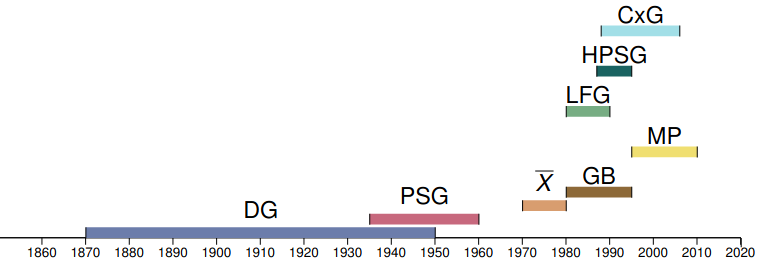
\includegraphics[scale=0.15]{historical-perspective.png}\\
\scriptsize{Dependency Grammar(DG)} {\tiny Most basic syntactic concepts (headedness, valency, POS, grammatical functions) were already relevant}\\
\scriptsize{Phrase Structure Grammar(PSG)} {\tiny added a strong constituency component via re-write rules. This also gave rise to tree and bracket representations}\\
\scriptsize{X-bar Theory} {\tiny took PSGs to a higher level of abstraction by introducing X-bar-rules}\\
\scriptsize{Government \& Binding(GB)} {\tiny tendency of further abstracting away from surface structure to understand deep structure was followed up. The principle of government is introduced to deal with case assignment, while binding deals with anaphora resolution. The field quickly fragmented into different definitions of such principles}\\
\scriptsize{Minimalist Program(MP)} {\tiny strongly reduces the GB aparatus in order to base syntactic theory on a few core operations (i.e. merge and move). Another divergence from GB and X-bar theory is that it uses features for structure building (rather than phrase structure rules)}\\
\scriptsize{Lexical Functional Grammar(LFG), Head-Driven Structure Grammar(HPSG)} {\tiny focus on lexicalization of syntactic structure by introducing feature descriptions in matrix form. This also rendered tree/bracket notations rather marginal}\\
\scriptsize{Construction Grammar} {\tiny breaks with a core concept of syntax, and promotes moving away from compositionality towards holistic patterns, i.e. constructions, which are learned and stored if sufficiently frequent.}\\
\scriptsize{Syntactic Framework Tree:}\\
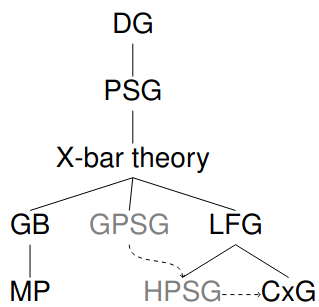
\includegraphics[scale=0.15]{syntactic_framework.png}\\
\scriptsize{Basic Concepts:}\\
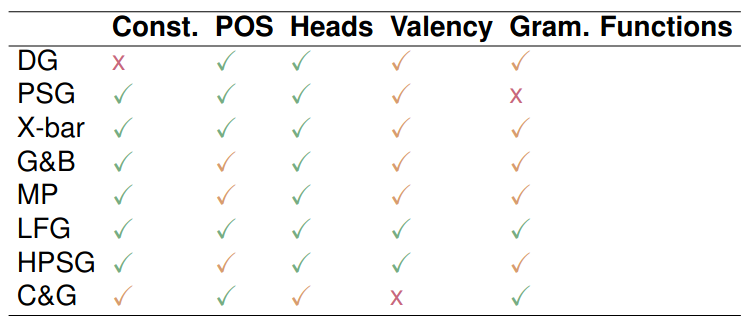
\includegraphics[scale=0.18]{basic-concepts.png}
\scriptsize{Transformational Framework} {\tiny there is some underlying template (i.e. deep structure) which is adapted by transformations and movements to give rise to the full variety of sentence structures encountered in linguistic production (except for noise such as misspronunciations)}\\
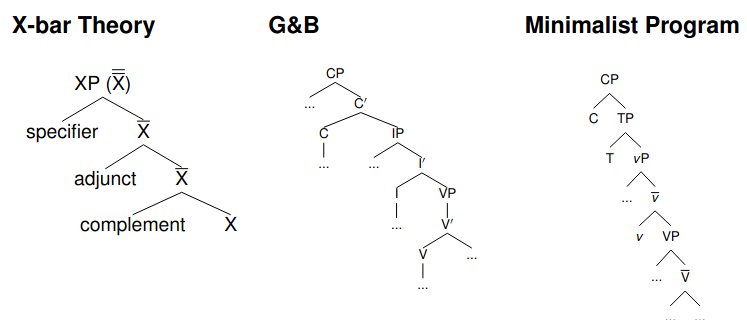
\includegraphics[scale=0.15]{transformational-framework.png}
\scriptsize{Constraint-Based Framework} {\tiny capture syntactic relationships by structural frames (e.g. feature matrices, constructions) which constrain how elements can be combined and slots are filled}\\
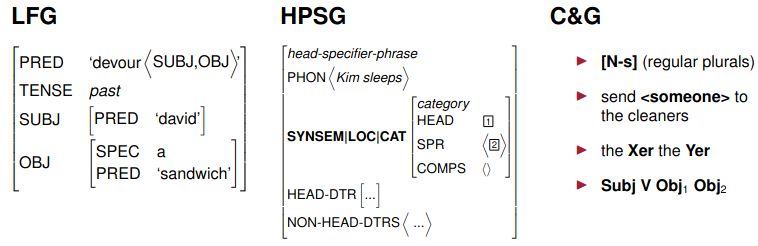
\includegraphics[scale=0.15]{constraint-based.png}
